\documentclass{standalone}
\usepackage{tikz}
\usetikzlibrary{patterns, positioning}
\usepackage[sfdefault]{ClearSans} %% option 'sfdefault' activates Clear Sans as the default text font
\usepackage[T1]{fontenc}

\begin{document}
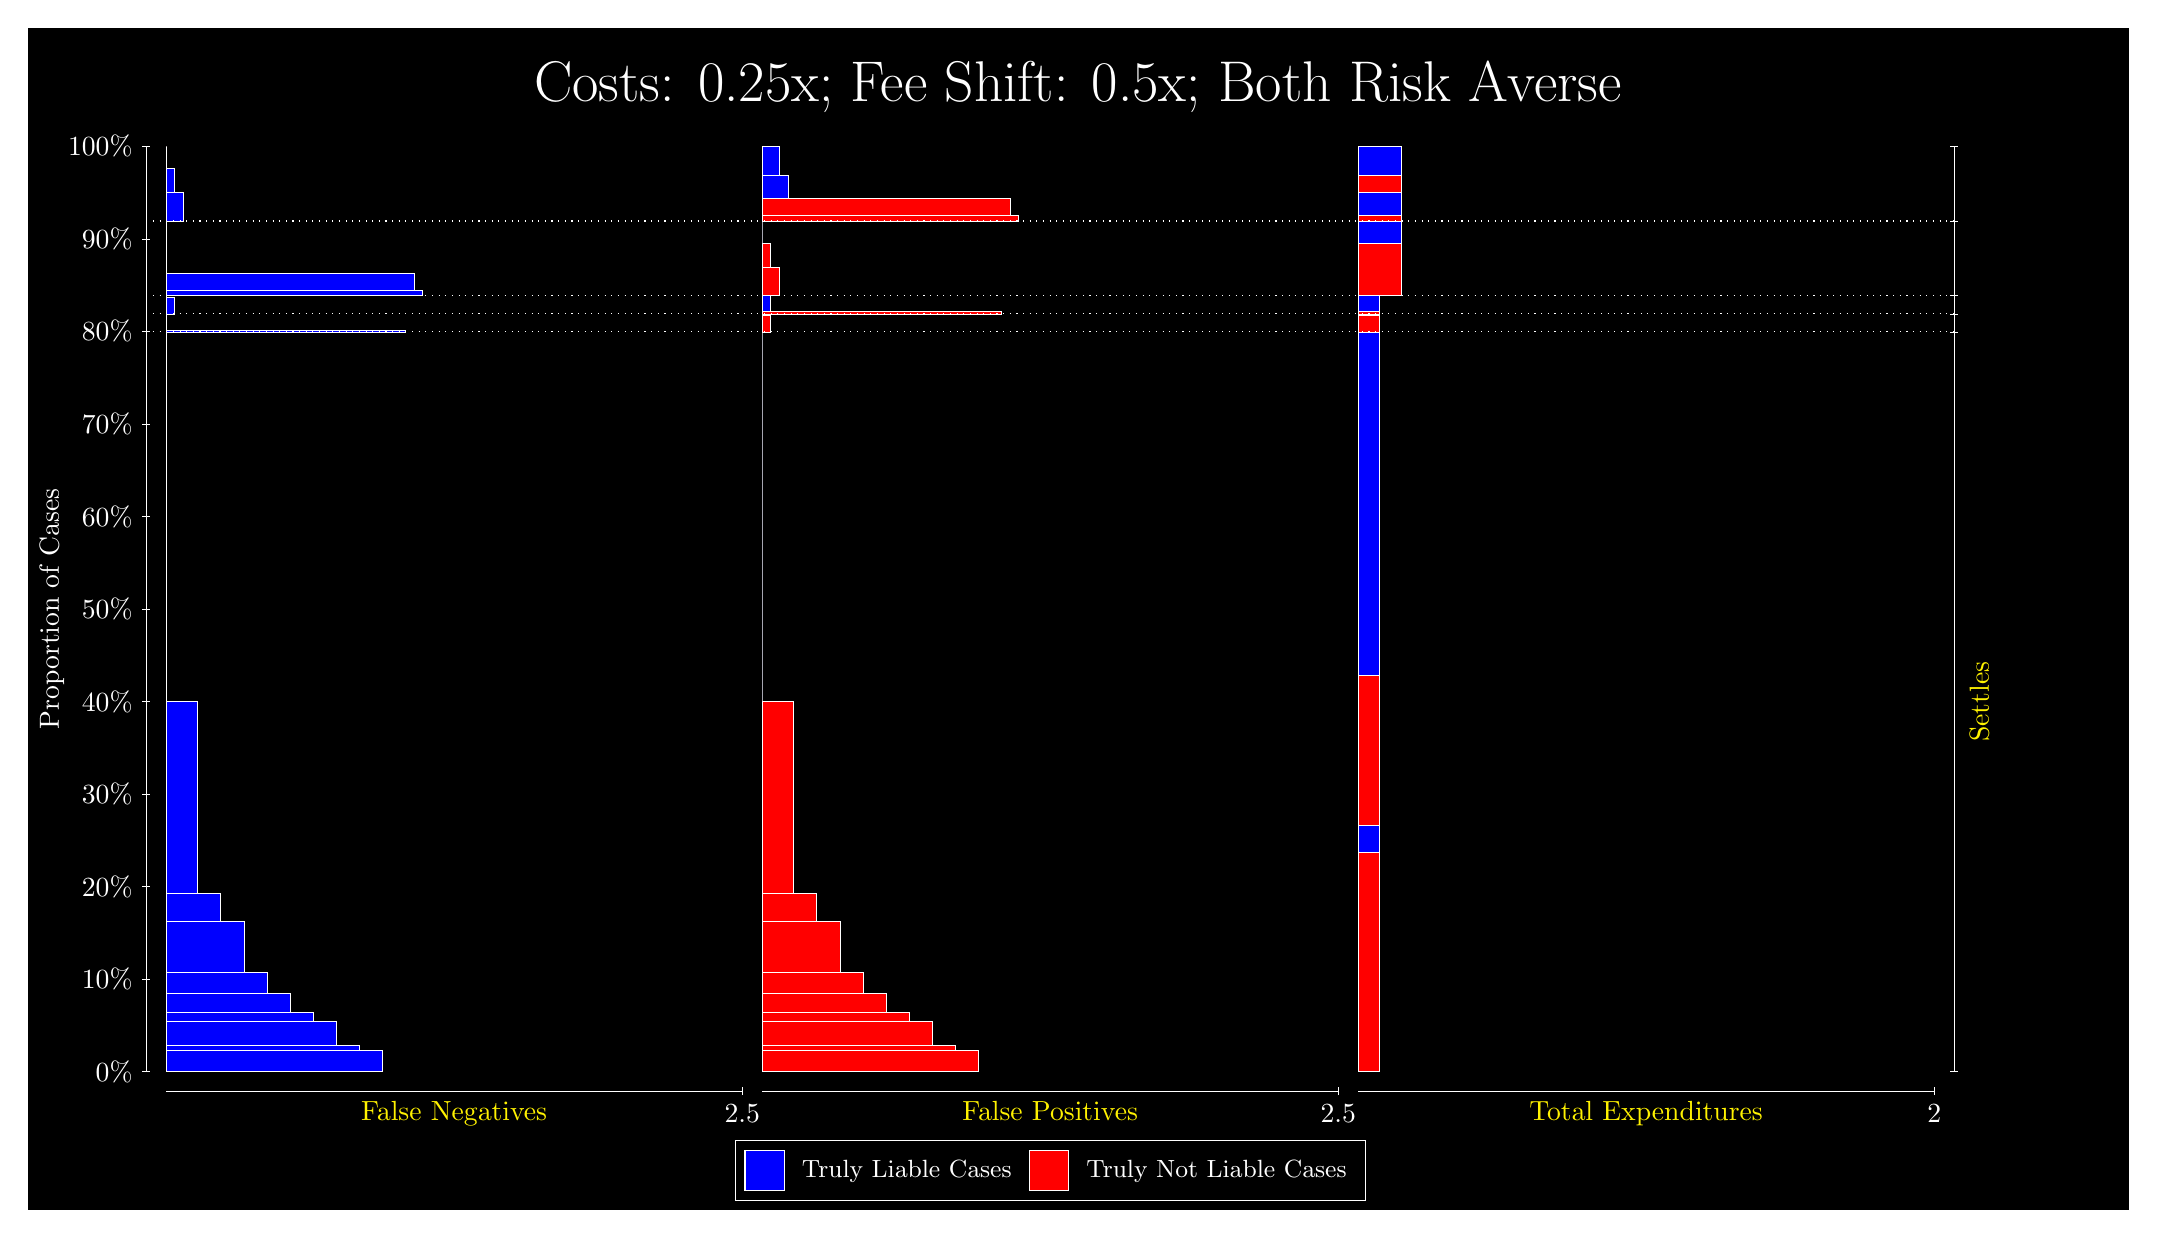
\begin{tikzpicture}
\draw[fill=black] (0,0) rectangle (26.667,15);
\draw[text=white] (0,13.5) rectangle (26.667,15) node[midway] {\huge Costs: 0.25x; Fee Shift: 0.5x; Both Risk Averse};
\draw[white, very thin] (1.5,1.75) -- (1.5,13.5);
\node[rotate=90, text=white, anchor=center] at (0.3, 7.625) {Proportion of Cases};
\draw[white, very thin] (1.45,1.75) -- (1.55,1.75);
\node[text=white, anchor=east] at (1.45, 1.75) {0\%};
\draw[white, very thin] (1.45,2.925) -- (1.55,2.925);
\node[text=white, anchor=east] at (1.45, 2.925) {10\%};
\draw[white, very thin] (1.45,4.1) -- (1.55,4.1);
\node[text=white, anchor=east] at (1.45, 4.1) {20\%};
\draw[white, very thin] (1.45,5.275) -- (1.55,5.275);
\node[text=white, anchor=east] at (1.45, 5.275) {30\%};
\draw[white, very thin] (1.45,6.45) -- (1.55,6.45);
\node[text=white, anchor=east] at (1.45, 6.45) {40\%};
\draw[white, very thin] (1.45,7.625) -- (1.55,7.625);
\node[text=white, anchor=east] at (1.45, 7.625) {50\%};
\draw[white, very thin] (1.45,8.8) -- (1.55,8.8);
\node[text=white, anchor=east] at (1.45, 8.8) {60\%};
\draw[white, very thin] (1.45,9.975) -- (1.55,9.975);
\node[text=white, anchor=east] at (1.45, 9.975) {70\%};
\draw[white, very thin] (1.45,11.15) -- (1.55,11.15);
\node[text=white, anchor=east] at (1.45, 11.15) {80\%};
\draw[white, very thin] (1.45,12.325) -- (1.55,12.325);
\node[text=white, anchor=east] at (1.45, 12.325) {90\%};
\draw[white, very thin] (1.45,13.5) -- (1.55,13.5);
\node[text=white, anchor=east] at (1.45, 13.5) {100\%};

\draw[white, very thin] (24.457,1.75) -- (24.457,13.5);
\draw[white, very thin] (24.407,1.75) -- (24.507,1.75);
\node[anchor=west] at (24.407, 1.75) {};
\draw[white, very thin] (24.407,11.143) -- (24.507,11.143);
\node[anchor=west] at (24.407, 11.143) {};
\draw[white, very thin] (24.407,11.373) -- (24.507,11.373);
\node[anchor=west] at (24.407, 11.373) {};
\draw[white, very thin] (24.407,11.604) -- (24.507,11.604);
\node[anchor=west] at (24.407, 11.604) {};
\draw[white, very thin] (24.407,12.552) -- (24.507,12.552);
\node[anchor=west] at (24.407, 12.552) {};
\draw[white, very thin] (24.407,13.5) -- (24.507,13.5);
\node[anchor=west] at (24.407, 13.5) {};

\draw[white, very thin, fill=blue] (1.75,1.75) rectangle (4.4946,2.0234);
\draw[white, very thin, fill=blue] (1.75,2.0234) rectangle (4.2018,2.0883);
\draw[white, very thin, fill=blue] (1.75,2.0883) rectangle (3.9091,2.3863);
\draw[white, very thin, fill=blue] (1.75,2.3863) rectangle (3.6163,2.4996);
\draw[white, very thin, fill=blue] (1.75,2.4996) rectangle (3.3236,2.743);
\draw[white, very thin, fill=blue] (1.75,2.743) rectangle (3.0308,3.0044);
\draw[white, very thin, fill=blue] (1.75,3.0044) rectangle (2.738,3.6557);
\draw[white, very thin, fill=blue] (1.75,3.6557) rectangle (2.4453,4.0191);
\draw[white, very thin, fill=blue] (1.75,4.0191) rectangle (2.1525,6.4463);
\draw[white, very thin, fill=red] (1.75,6.4463) rectangle (1.75,11.143);
\draw[white, very thin, fill=blue] (1.75,11.143) rectangle (4.7873,11.168);
\draw[white, very thin, fill=red] (1.75,11.168) rectangle (1.75,11.373);
\draw[white, very thin, fill=blue] (1.75,11.373) rectangle (1.8598,11.578);
\draw[white, very thin, fill=red] (1.75,11.578) rectangle (1.75,11.604);
\draw[white, very thin, fill=blue] (1.75,11.604) rectangle (5.0069,11.67);
\draw[white, very thin, fill=blue] (1.75,11.67) rectangle (4.8971,11.886);
\draw[white, very thin, fill=red] (1.75,11.886) rectangle (1.75,12.552);
\draw[white, very thin, fill=blue] (1.75,12.552) rectangle (1.9696,12.915);
\draw[white, very thin, fill=blue] (1.75,12.915) rectangle (1.8598,13.218);
\draw[white, very thin, fill=red] (1.75,13.218) rectangle (1.75,13.5);
\draw[white, very thin, fill=red] (9.3189,1.75) rectangle (12.063,2.0234);
\draw[white, very thin, fill=red] (9.3189,2.0234) rectangle (11.771,2.0883);
\draw[white, very thin, fill=red] (9.3189,2.0883) rectangle (11.478,2.3862);
\draw[white, very thin, fill=red] (9.3189,2.3862) rectangle (11.185,2.4996);
\draw[white, very thin, fill=red] (9.3189,2.4996) rectangle (10.892,2.743);
\draw[white, very thin, fill=red] (9.3189,2.743) rectangle (10.6,3.0044);
\draw[white, very thin, fill=red] (9.3189,3.0044) rectangle (10.307,3.6558);
\draw[white, very thin, fill=red] (9.3189,3.6558) rectangle (10.014,4.0192);
\draw[white, very thin, fill=red] (9.3189,4.0192) rectangle (9.7214,6.4464);
\draw[white, very thin, fill=blue] (9.3189,6.4464) rectangle (9.3189,11.143);
\draw[white, very thin, fill=red] (9.3189,11.143) rectangle (9.4287,11.348);
\draw[white, very thin, fill=blue] (9.3189,11.348) rectangle (9.3189,11.373);
\draw[white, very thin, fill=red] (9.3189,11.373) rectangle (12.356,11.399);
\draw[white, very thin, fill=blue] (9.3189,11.399) rectangle (9.4287,11.604);
\draw[white, very thin, fill=red] (9.3189,11.604) rectangle (9.5384,11.967);
\draw[white, very thin, fill=red] (9.3189,11.967) rectangle (9.4287,12.269);
\draw[white, very thin, fill=blue] (9.3189,12.269) rectangle (9.3189,12.552);
\draw[white, very thin, fill=red] (9.3189,12.552) rectangle (12.576,12.618);
\draw[white, very thin, fill=red] (9.3189,12.618) rectangle (12.466,12.834);
\draw[white, very thin, fill=blue] (9.3189,12.834) rectangle (9.6482,13.137);
\draw[white, very thin, fill=blue] (9.3189,13.137) rectangle (9.5384,13.5);
\draw[white, very thin, fill=red] (16.888,1.75) rectangle (17.162,4.5407);
\draw[white, very thin, fill=blue] (16.888,4.5407) rectangle (17.162,4.879);
\draw[white, very thin, fill=red] (16.888,4.879) rectangle (17.162,6.7848);
\draw[white, very thin, fill=blue] (16.888,6.7848) rectangle (17.162,11.143);
\draw[white, very thin, fill=red] (16.888,11.143) rectangle (17.162,11.348);
\draw[white, very thin, fill=blue] (16.888,11.348) rectangle (17.162,11.373);
\draw[white, very thin, fill=red] (16.888,11.373) rectangle (17.162,11.399);
\draw[white, very thin, fill=blue] (16.888,11.399) rectangle (17.162,11.604);
\draw[white, very thin, fill=red] (16.888,11.604) rectangle (17.437,12.269);
\draw[white, very thin, fill=blue] (16.888,12.269) rectangle (17.437,12.552);
\draw[white, very thin, fill=red] (16.888,12.552) rectangle (17.437,12.618);
\draw[white, very thin, fill=blue] (16.888,12.618) rectangle (17.437,12.921);
\draw[white, very thin, fill=red] (16.888,12.921) rectangle (17.437,13.137);
\draw[white, very thin, fill=blue] (16.888,13.137) rectangle (17.437,13.5);
\draw[white, dotted] (1.5,11.143) -- (24.457,11.143);
\draw[white, dotted] (1.5,11.373) -- (24.457,11.373);
\draw[white, dotted] (1.5,11.604) -- (24.457,11.604);
\draw[white, dotted] (1.5,12.552) -- (24.457,12.552);
\draw[white, very thin] (1.75,1.5) -- (9.0689,1.5);
\node[text=yellow, anchor=north] at (5.4094, 1.5) {False Negatives};
\draw[white, very thin] (9.0689,1.45) -- (9.0689,1.55);
\node[text=white, anchor=north] at (9.0689, 1.45) {2.5};

\draw[white, very thin] (9.3189,1.5) -- (16.638,1.5);
\node[text=yellow, anchor=north] at (12.978, 1.5) {False Positives};
\draw[white, very thin] (16.638,1.45) -- (16.638,1.55);
\node[text=white, anchor=north] at (16.638, 1.45) {2.5};

\draw[white, very thin] (16.888,1.5) -- (24.207,1.5);
\node[text=yellow, anchor=north] at (20.547, 1.5) {Total Expenditures};
\draw[white, very thin] (24.207,1.45) -- (24.207,1.55);
\node[text=white, anchor=north] at (24.207, 1.45) {2};

\node[text=yellow, centered, rotate=90] at (24.777, 6.4464) {Settles};





\draw (12.978300999999998,1.5) node[draw=none] (baseCoordinate) {};
\begin{scope}[align=center]
        \matrix[scale=0.5, draw=white, below=0.5cm of baseCoordinate, nodes={draw}, column sep=0.1cm]{
            \node[rectangle, draw, minimum width=0.5cm, minimum height=0.5cm, fill=blue] {}; &
            \node[draw=none, font=\small, text=white] (B) {Truly Liable Cases}; &
            \node[rectangle, draw, minimum width=0.5cm, minimum height=0.5cm, fill=red] {}; &
            \node[draw=none, font=\small, text=white] (B) {Truly Not Liable Cases}; \\
            };
\end{scope}

\end{tikzpicture}
\end{document}